\nsecbegin{Ziel des Sprints}
Die bestehenden Funktionen des Programms sollen um die Möglichkeit ergänzt werden, neben Klassendiagrammen auch Sequenzdiagramme erstellen zu können. Dafür muss die Struktur der verarbeiteten Daten, also auch der Code zum Parsen, angepasst werden. Geplant ist eine Repräsentation des eingelesenen Codes als zentrale XML-Datei, die je nach Anwendungszweck wiederum die Basis für zwei unterschiedliche XML-Dateien ist.

% HIER NEUES KLASSENDIAGRAMM HINZUFUEGEN
%\begin{figure}[hbtp]
%\centering
%\includegraphics[scale=0.5]{}
%\caption{Klassendiagramm des Sprints}
%\end{figure}
%\nsecend

\nsecbegin{User-Stories des Sprint-Backlogs}
\nsecbegin{Sequenzdiagramme}
\nsecbegin{Auswahl des zu erstellenden Diagramms}
Als Benutzer wünsche ich mir, dass eine Auswahl zwischen Klassen- und Sequenzdiagrammen möglich ist, damit ich diese je nach meinen Bedürfnissen generieren kann.
\nsecend

\nsecbegin{Generierung von Sequenzdiagrammen}
Als Benutzer wünsche ich mir, Sequenzdiagramme erstellen zu können, um einen Überblick über die Abläufe meines Programms zu erhalten.
\nsecend
\nsecend%Sequenzdiagramme

\nsecbegin{Interne Struktur}
\nsecbegin{Parserfunktionalität}
Als Softwarearchitekt wünsche ich mir, dass der Parser effizient funktioniert, um die benötigten Daten ohne Schwierigkeiten auszulesen.
\nsecend

\nsecbegin{Dateiformat XML}
Als Softwarearchitekt wünsche ich mir, dass der übergebene Code zur weiteren Verarbeitung in verschiedene XML-Dateien umgewandelt wird.
\nsecend
\nsecend%Interne Struktur
\nsecend % {User-Stories des Sprint-Backlogs}

\nsecbegin{Zeitliche Planung}
\begin{figure}[hbtp]
\centering
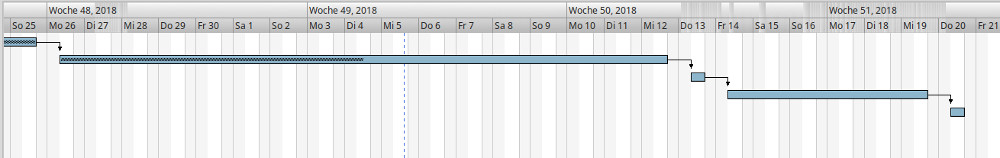
\includegraphics[width=\textwidth]{Bilder/gantt}
\caption{Gantt-Diagramm für Sprint 1}
\end{figure}
\nsecend%Zeitliche Planung

\nsecbegin{Liste der durchgeführten Meetings}
\begin{itemize}
\item Planning-Meeting (15.04.2019)
\item Parser-Besprechung (18.04.2019)
\item Parser-Besprechung (24.04.2019)
\item Zwischen-Meeting (25.04.2019)
\item Review-Meeting (29.4.2019)
\end{itemize}
\nsecend%Liste der durchgeführten Meetings

\nsecbegin{Ergebnisse des Planning-Meetings}
Dem gesamten Team ist die geplante Grundstruktur des Programms bekannt. Jeder weiß, welcher Teil des Programms zu implementieren ist.
\nsecend

\nsecbegin{Aufgewendete Arbeitszeit pro Person$+$Arbeitspaket}
\begin{longtable}{|p{4cm}|l|l|l|l|l|}
        \hline
        Arbeitspaket & Person & Start & Ende & h & Artefakt\\
        \hline
        Dummyklassen & Musterstudi & 3.5.09 & 12.5.09 & 14 & Klasse.java\\ \hline
        AP XYZ &  &  &  & & \\ \hline
\end{longtable}     
\nsecend

\nsecbegin{Konkrete Code-Qualität im Sprint}
Die Code-Qualität ist bisher gleichmäßig. Da die Umstrukturierung des Parsers besondere Sorgfalt erfordert, wurden zusätzliche Treffen mit den verantwortlichen Teammitgliedern angesetzt.
\nsecend%Konkrete Code-Qualität im Sprint

\nsecbegin{Konkrete Test-Überdeckung im Sprint}
Die Test-Überdeckung in diesem Sprint fiel eher niedrig aus, da für die neuen Funktionen erst passende Testdateien erstellt bzw. bestehende Testdateien angepasst werden müssen.
\nsecend%Konkrete Test-Überdeckung im Sprint

\nsecbegin{Ergebnisse des Reviews}
\begin{table}[H]

\begin{tabularx}{\textwidth}{ |l|l|X| }
\hline
\textbf{Klasse} & \textbf{Methode} & \textbf{Anmerkungen}\\
 \hline
%Console & showConsole & Pfad anpassen \\
\hline
\end{tabularx}
\end{table}

Sonstiges:
\begin{itemize}
\item Zum Testen des überarbeiteten Parsers müssen die Testdateien angepasst werden
\end{itemize}
\nsecend%Ergebnisse des Reviews

\nsecbegin{Ergebnisse der Retrospektive}
Die Retrospektive schloss mit einer gemischten Bilanz. Besonders die Umstrukturierung des Parsers warf viele Fragen auf, da nicht nur der Code des Parsers selbst, sondern auch alle Schnittstellen angepasst werden mussten. Hier zeichnete sich eine leichte Unzufriedenheit ab, da Teile der bisher geleisteten Arbeit nun umgeschrieben werden. Für den nächsten Sprint ist es daher wünschenswert, die Erzeugung der neuen XML-Dateien sowie darauf aufbauend der Sequenzdiagramme voranzutreiben, damit hier möglichst bald ein Erfolg zu verzeichnen ist.
\nsecend%Ergebnisse der Retrospektive

\nsecbegin{Abschließende Einschätzung des Product-Owners}
Insgesamt ist ein beachtlicher Teil der definierten Sprintziele noch in Bearbeitung. Da es sich um einen kurzen Sprint handelte und zudem große Teile des Codes geändert werden müssen, um die Generation von Sequenzdiagrammen vorzubereiten, ist dies nachvollziehbar. 
\nsecend%Abschließende Einschätzung des Product-Owners

\nsecbegin{Abschließende Einschätzung des Software-Architekten}
XXX
\nsecend%Abschließende Einschätzung des Software-Architekten

\nsecbegin{Abschließende Einschätzung des Team-Managers}
Vom allgemeinen Sprintverlauf ausgehend wird das Erstellen von Sequenzdiagrammen die größte Herausforderung des Projekts werden. Damit die betreffenden Teammitglieder im Vergleich nicht zu viel Zeit in den Parser investieren müssen, wurden zwei zusätzliche Treffen mit dem Softwarearchitekten angesetzt, bei denen die notwendigen Voraussetzungen besprochen und die Methodik erörtert wurde.
\nsecend%Abschließende Einschätzung des Team-Managers